\begin{figure}[htbp]
    \centering
    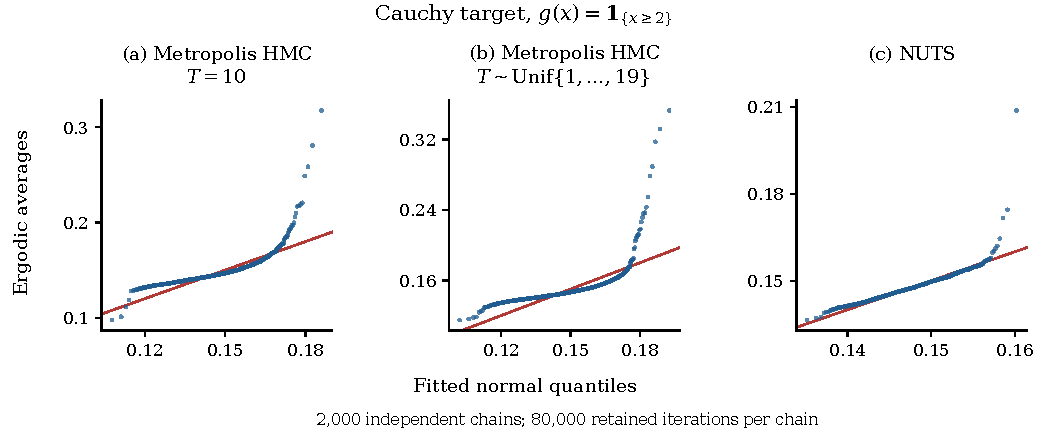
\includegraphics[width=\textwidth]{figures/03_hmc_nuts.pdf}
    \caption{Cauchy tail-probability averages under Metropolis-adjusted HMC
    with $T=10$, Metropolis-adjusted HMC with independent
    $T\sim\mathrm{Unif}\{1,\ldots,19\}$ at each iteration, and NUTS.
    NUTS uses BlackJAX 1.6.2 with JAX 0.11.2, standard trajectory
    construction and its library defaults, with no adaptation.
    All methods use the fixed step size, unit mass, replication, burn-in
    and raw Gaussian QQ construction of Figure~\ref{fig:ula-fixed-random}.
    Iteration counts are equal; gradient costs differ.
    The plots compare finite-run distributional shape and do not establish
    polynomial convergence rates or CLT failure for NUTS.}
    \label{fig:hmc-nuts}
\end{figure}
